\documentclass[10pt,a4paper]{article}
\usepackage[utf8]{inputenc}
\usepackage[T1]{fontenc}
\usepackage{fullpage}
\usepackage{amsfonts,amsmath,amssymb,mathtools, bm}
\usepackage{comment,color, fancybox}
\usepackage{verbatim}
\usepackage{enumitem}
\usepackage{listings}
\usepackage{xcolor}
\usepackage{array}
\usepackage{ragged2e}
\usepackage{csvsimple}
\usepackage{changepage}
% \usepackage[alf]{ABNTex/abntex2cite}
\usepackage[ddmmyyyy]{datetime}

\lstset{language=C++,
	basicstyle=\ttfamily,
	keywordstyle=\color{blue}\ttfamily,
	stringstyle=\color{green}\ttfamily,
	commentstyle=\color{gray}\ttfamily,
	morecomment=[l][\color{magenta}]{\#}
}

\newcommand{\ttt}[1]{\texttt{#1}}

\title{Relatório do Desempenho de Aplicações Paralelas Usando OpenMP} 
\author{Miguel Nunes}
\date{\today}

\begin{document}
	\maketitle

	\section{Algoritmos e Descrição do Ambiente}

		Foi analisado o algoritmos de Mandelbrot paralelizado usando Open MP e MPI, 
		com apenas leves modificações na entrada de dados e alocação de memória para facilitar a automatização dos testes.
		Foram utilizadas os valores como entrada: 
		
		\begin{verbatim}
			max_row    = 340
			max_column = 1000
			max_n      = 4600
		\end{verbatim}

		Pois foi observado experimentalmente que, em execuções sequenciais do algoritmo, essas entradas levavam, em média, 
		64 segundos para serem processadas.

		Os testes foram realizados nos servidores \texttt{ens1}, \texttt{ens2} e \texttt{ens4} disponibilizados pelo professor e
		foram executados automaticamente a partir de um script em bash, com o auxílio de um makefile.

	\section{Coleta dos Dados}
		O algoritmo usando MPI foi executado em 12 processos, 4 processos em cada servidor, já o algoritmo usando Open MP foi executado
		com 4 threads em cada servidor.
		Ao fim da execução dos algoritmos, o tempo de execução é imprimida para \texttt{stdout}. 
		Nos testes \texttt{stdout} era redirecionado para um arquivo de texto por meio de operações de \textit{pipe} do bash.

		Foram feitas 10 execuções de cada algoritmo, com os seguintes resultados de tempo de execução:

		\clearpage

		\begin{table}[htb]
			\centering
			\begin{tabular}{|c|c|}
				\hline
				Execução & Tempo de Execução\\ \hline
				1  & 11.474648 \\ \hline
				2  & 11.559622 \\ \hline
				3  & 11.450598 \\ \hline
				4  & 11.610346 \\ \hline
				5  & 11.499296 \\ \hline
				6  & 11.464533 \\ \hline
				7  & 11.526878 \\ \hline
				8  & 11.562462 \\ \hline
				9  & 11.513563 \\ \hline
				10 & 11.513563 \\ \hline
			\end{tabular}
			\caption{Mandelbrot com Open MP em \texttt{ens1}}
		\end{table}
		Média = \texttt{11.514} segundos, Desvio Padrão = \texttt{0.050804}.

		\begin{table}[htb]
			\centering
			\begin{tabular}{|c|c|}
				\hline
				Execução & Tempo de Execução\\ \hline
				1  & 11.953199 \\ \hline
				2  & 11.525896 \\ \hline
				3  & 11.584578 \\ \hline
				4  & 11.575379 \\ \hline
				5  & 11.574743 \\ \hline
				6  & 11.569756 \\ \hline
				7  & 11.664425 \\ \hline
				8  & 11.585252 \\ \hline
				9  & 11.739646 \\ \hline
				10 & 11.77709 \\ \hline
			\end{tabular}
			\caption{Mandelbrot com Open MP em \texttt{ens2}}
		\end{table}
		Média = \texttt{11.654} segundos, Desvio Padrão = \texttt{0.132338}.

		\begin{table}[htb]
			\centering
			\begin{tabular}{|c|c|}
				\hline
				Execução & Tempo de Execução\\ \hline
				1  & 5.6473 \\ \hline
				2  & 5.6755 \\ \hline
				3  & 5.5199 \\ \hline
				4  & 5.5874 \\ \hline
				5  & 5.4372 \\ \hline
				6  & 5.5894 \\ \hline
				7  & 5.6809 \\ \hline
				8  & 5.5273 \\ \hline
				9  & 5.5947 \\ \hline
				10 & 5.7734 \\ \hline
			\end{tabular}
			\caption{Mandelbrot com Open MP em \texttt{ens4}}
		\end{table}
		Média = \texttt{5.603} segundos, Desvio Padrão = \texttt{0.096000}.

		\clearpage

		\begin{table}[htb]
			\centering
			\begin{tabular}{|c|c|}
				\hline
				Execução & Tempo de Execução\\ \hline
				1  & 4.8423 \\ \hline
				2  & 4.9263 \\ \hline
				3  & 4.9343 \\ \hline
				4  & 4.8407 \\ \hline
				5  & 4.8459 \\ \hline
				6  & 4.8148 \\ \hline
				7  & 4.8427 \\ \hline
				8  & 4.8440 \\ \hline
				9  & 4.8720 \\ \hline
				10 & 4.8746 \\ \hline
			\end{tabular}
			\caption{Mandelbrot com MPI}
		\end{table}
		Média = \texttt{4.863} segundos, Desvio Padrão = \texttt{0.038894}.

	\section{Análise do Dados}

		Analisando os resultados de tempo de execução e o gráfico abaixo podemos observar que o teste com MPI
		teve desempenho consideravelmente superior que os testes com Open MP, porém a diferença não foi tão
		grande quando comparada com o teste em Open MP rodado no servidor \texttt{ens4}, que tem \textit{hardware}
		consideravelmente melhor que os outros dois servidores.
		
		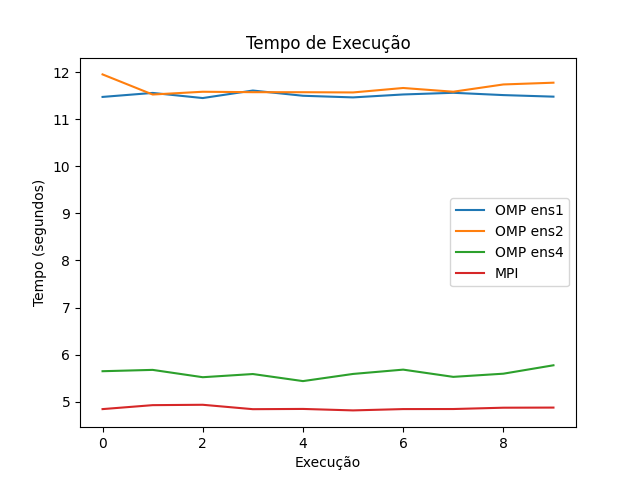
\includegraphics[scale=.7]{Tempo.png}
		
		Podemos então concluir que MPI consegue ter um desempenho melhor em situações onde há diversos computadores
		com \textit{hardware} de baixo desempenho, porém não consegue um desempenho ideal em situações onde há
		computadores com \textit{hardware} de alto e baixo desempenho misturados numa rede. 
		
		Isso é evidente comparando os resultados do caso de Open MP em \texttt{ens4} e o caso de MPI. Apesar do algoritmo
		rodando MPI estar rodando 4 processos em 3 computadores distintos, ele teve um tempo médio de execução apenas
		\texttt{0.8} segundos menor que o caso do Open MP naquele servidor, o que indica que o MPI não conseguiu se aproveitar
		totalmente dos recursos de \texttt{ens4}.

		Ao mesmo tempo, o teste em Open MP nesse servidor poderia ter desempenho melhor, já que apenas 4 das 8 threads disponíveis
		foram utilizadas. 
\end{document}